\documentclass[12pt]{article}
\usepackage{amsmath}
\usepackage{amssymb}
%\usepackage[margin=1.2 in, includefoot]{geometry}
\usepackage{color}
\usepackage{rotating}
%\usepackage{setspace}
\usepackage{graphicx}
\author{Zimian Zhang}
\title{Dynamic Models of Cash Management: the 2nd Year's Report}
\begin{document}

%\begin{spacing}{1.0}
\maketitle
\setcounter{page}{0}
\thispagestyle{empty}


\newpage
\tableofcontents
\setcounter{page}{0}
\thispagestyle{empty}

\newpage

\section {Introduction}

Cash management deals with the company's cash holding strategy. With insufficient cash holding level, a company might expose to the risk of cash deficit, which might cause a great amount of penalty. On the other hand, a high cash-holding level normally means the inefficient use of firm's resource, which would constrain firm's future profitability. The ultimate goal of studying cash management problem is to propose a policy to maximise the firm's profitability while minimising the damage caused by cash deficit.

Many studies in cash management adopt the `one asset account'  setting (e.g. \cite{baccarin2002optimal}, \cite{sato2011stochastic}, \cite{bensoussan2005optimality} and \cite{feng2010computational}). In these studies, only the cash account is considered. In each time period, managers can adjust the cash holding level with some transfer fee. Meanwhile, the company will face a certain amount of cash demand. If the current cash holdings cannot meet the cash demand, shortage cost occurs. On the other hand, a positive cash holdings will also generate some opportunity cost, that is the profits one could get had the manager invested the cash into a profitable asset. The basic idea of `one asset account' models is shown in figure \ref{basic model}. The limitation of these models is that both cash flows are considered exogenous, i.e. cash outflows or inflows will not be affected by the policies taken by decision-makers. 


In light of this, we proposed a two-assets cash management (CM) model in our first year's research (see figure \ref{twoAsset}). In this model, managers can transfer any amount of money between cash account and asset account with a fixed amount of transaction fee ($\Gamma$). We assumed that at the beginning of each time period, the company will receive some cash as business revenue which is proportional to the current size of its profitable asset ($BR = rr \cdot y_t$). Moreover during each time period, a stochastic amount of cash demand occurs ($D$). If the cash demand exceeds current cash holdings, managers have to sell their asset to offset the cash deficit along with a fixed amount of cash shortage penalty ($SC$). The objective function of this model is to maximise the total cash inflow for an infinite time horizon. 

The advantage of this model is that the size of cash inflow are affected by managers actions and that the profit of investing money into business rather than holding as cash is compounded over time. Figure \ref{firstY} shows one result of this model. It shows the different cash actions the manager should take given his company is in the corresponding states. An action with positive values indicates to transfer that amount of money from the asset account to the cash account and an action with negative values means moving money the other way around. 



\begin{figure}
\begin{center}
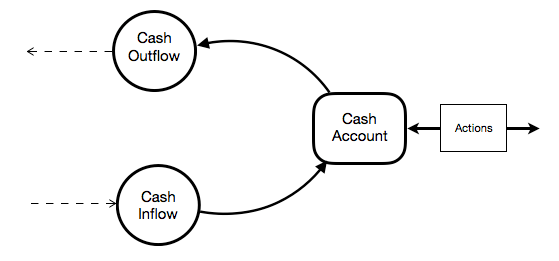
\includegraphics[scale=.4]{basicModel}
\end{center}
\caption{One Asset CM Model}
\label{basic model}
\end{figure}

\begin{figure}
\begin{center}
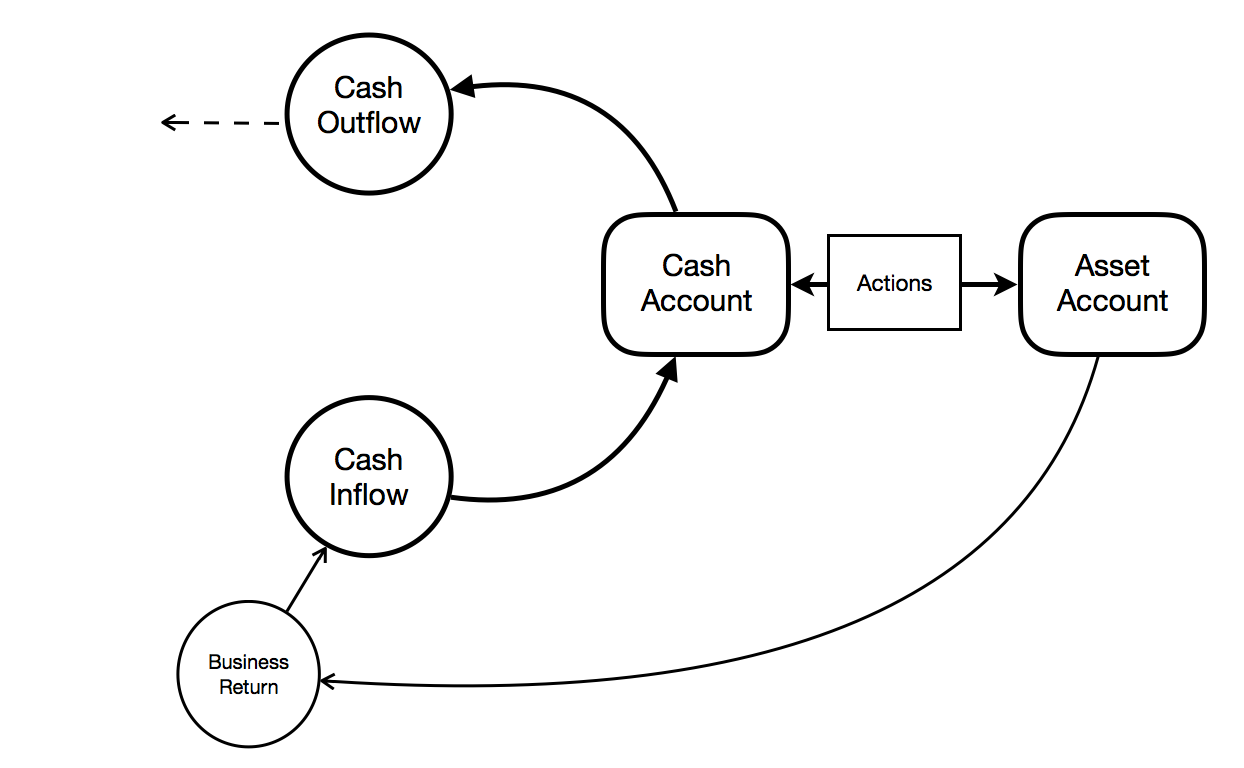
\includegraphics[scale=.35]{twoAssets}
\end{center}
\caption{Two Assets CM Model}
\label{twoAsset}
\end{figure}



\begin{figure}
\begin{center}
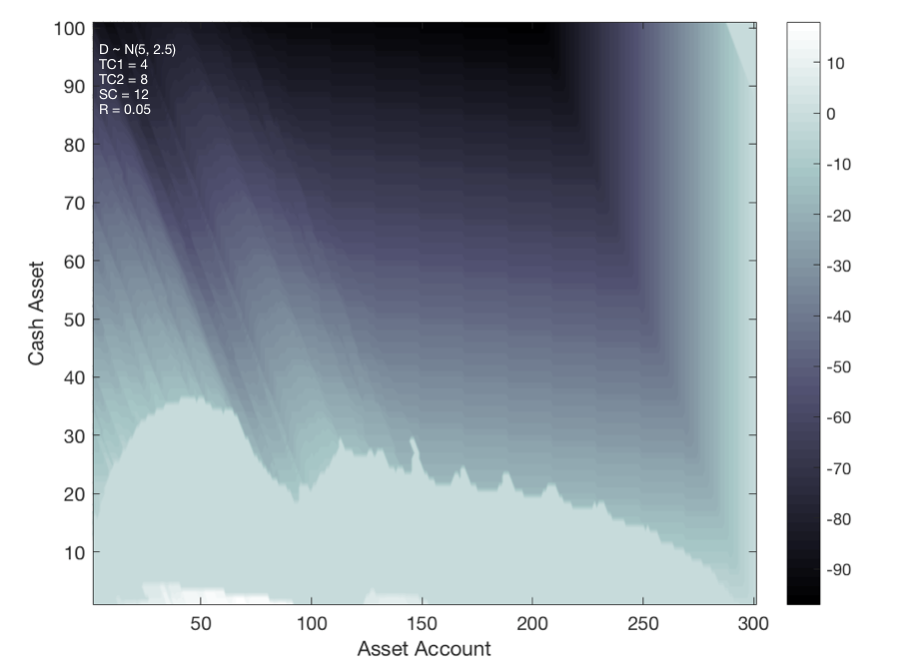
\includegraphics[scale=.25]{ResultFirstYear_rdy}
\end{center}
\caption{A Optimal Solution of the Two Accounts Model}
\label{firstY}
\end{figure}

This document consists of three parts: a brief description of the overall research project, a summary of current progress and a plan for next year. In the next section, we will present the whole research project. To begin with, the motivation of my research will be discussed along with its potential contribution. Then each chapter of my thesis will be examined. At the end of this section we will discuss potential risks in this research.
Then we will present our work from last year and our current position of the whole research in section three. The work we have done mainly consists of four parts: a holistic cash management (CM) model in financial sector, a two-assets CM model, a CM model with loans or investments and the application of approximate dynamic programming (ADP) in CM models. In the fourth section we will give a research plan for next year as well as a time table. Moreover, we will give a summary of the courses and activities taken in last year and those will be taken in next year.


\section{Overall research project}
\subsection{Motivation and potential contribution}
While there is much literature on cash management problem, very few discussed the cash holding policy with the consideration of holistic cash flows inside a company. In our research, instead of considering it solitarily, we study the cash holding strategy with the activities of other cash flows. To be specific, we consider a company in financial sector in which the cash holding level strategy is affected by many other actions, such as taking loans from banks or other financial intermediaries, taking deposit from customers and spending money in capital assets. In the holistic model, the market environment factor will be taken into consideration as well. We propose this holistic model in the hope that it could help managers in financial industries control cash flows effectively and efficiently.

\subsection{Thesis structure}
There are many studies in cash management problem focusing on different details. For example Hinderer and Waldmann \cite{hinderer2001cash} studied cash management in a randomly varying environment, Nascimento, Juliana and Powell, Warren\cite{nascimento2010dynamic} present a cash management model in mutual funds company which recognise shareholder's redemptions as the source of cash demand, Bensoussan, Chutani and Sethi\cite{optimal} present a cash management model in which dividends and capital gains are the source of cash inflows. In light of these studies, we will propose a cash management model with a more holistic perspective which applies to financial companies. In our thesis, we first present this holistic model based on the literature. In order to solve this complicated model, we will start from a simple two assets CM model. We will show that dynamic programming method can solve the simple CM model with a reasonable computation cost. After that, we will complicate our model by taking loan opportunities into consideration. Moreover, we will present a heuristic method that gives a good approximate solution with much lower computation cost than dynamic programming. At last, we will adopt the approximate dynamic programming method in the hope that it could solve the holistic model efficiently. Our thesis should be organised as shown below:

\begin{itemize}
\item Chapter I.	Introduction
\item Chapter II. Literature Review
\begin{itemize}
\item  2.1 Literature Review of Cash Management in OR
\item  2.2 Literature Review of  Cash Flows in Financial Sector
\item 2.3 A Holistic Model based on Literature
\end{itemize}
\item Chapter III. Methodology
\begin{itemize}
\item  3.1 Introduction to Dynamic Programming
\item  3.2 Introduction to Approximate Dynamic Programming
\end{itemize}
\item Chapter IV. A Two Assets Cash Management Model
\begin{itemize}
\item  4.1 Model Summary
\item  4.2 Dynamic Programming Method
\item 4.3 Numeric Experiment
\end{itemize}

\item Chapter V. A Cash Management Model with Loans
\begin{itemize}
\item  5.1 Model Summary
\item  5.2 Dynamic Programming Method
\item  5.3 Heuristic Method: One Step Policy Improvement
\item  5.4 Numeric Experiment
\end{itemize}

\item Chapter VI. Approximate Dynamic Programming in Cash Management Model
\begin{itemize}
\item  6.1 Temporal Difference Method
\item  6.2 Eligibility Trace Method
\item  6.3 Function Approximation
\end{itemize}
\item Chapter VII. Conclusion
\end{itemize}

\subsection{Risk management}
The risk of our research are mainly from two aspects: the validation of the holistic model and the performance of approximate dynamic programming. As we mentioned before, the holistic model is a model based on literature. We design this model to fit situations in financial companies. However, there is no data to support our model. To justify this holistic model, further research are required. We are also concerned with the performance of approximate dynamic programming methods. So far we examined the performance of temporal difference method in the two assets CM model. But the converging speed is not satisfying. Currently we are using different step size and the eligibility trace method to improve the solution. But we cannot guarantee that approximate dynamic programming method can solve the holistic model effectively. Should the ADP failed to solve the model, studies of other problem-solving methods are required.


\section{Current progress}
\subsection{Holistic model: a CM model in financial sector}
Most literature in cash management problem consider the sources of cash outflows and inflows as exogenous random variables. But in the real world, cash flows in a company could easily affected each other and thus we propose a cash management model with a holistic consideration.
Figure \ref{Holistic} shows cash flows in a financial company(e.g. a commercial bank, a mutual fund or a pension fund company). To begin with, we consider capital asset and liquid asset separately. Liquid asset (such as portfolios or business investment) are those asset that can be relatively easily sold for cash. The returns from liquid asset is a source of cash inflow. In other words, the amount of liquid asset holdings can affect business income directly. Capital asset, on the other hand, are those assets that cannot be easily sold with a good price and do not affect companies profitability in short terms (e.g. branches, office equipments and employees). However, the capacities of holding liquid asset depends on the size of capital asset. For example, one broker can only serve a number of customers or a commercial bank are difficult to attract customers without a local branch. Meanwhile the capital asset generate another source of cash outflows: operation expense. For example, more office equipments require higher maintenance fees; a new branch office would cause higher utility bills and a company usually spend a lot of money to hire and train a new employee. Besides the cash inflows generated by liquid asset, a financial company could also take loans from other companies or take investment/deposit from customers. But loans would generate a fixed and predictable source of cash outflows: loan expense while customers' deposit would cause a random and unpredictable source of cash outflows: customers' redemption. Moreover, a exogenous variable, market environment, can affect the cash flows. For example, in a bear market, loan interest rate might increase, customers are more likely to withdraw their deposit and the return rate of liquid asset might decrease. 



\begin{figure}
\begin{center}
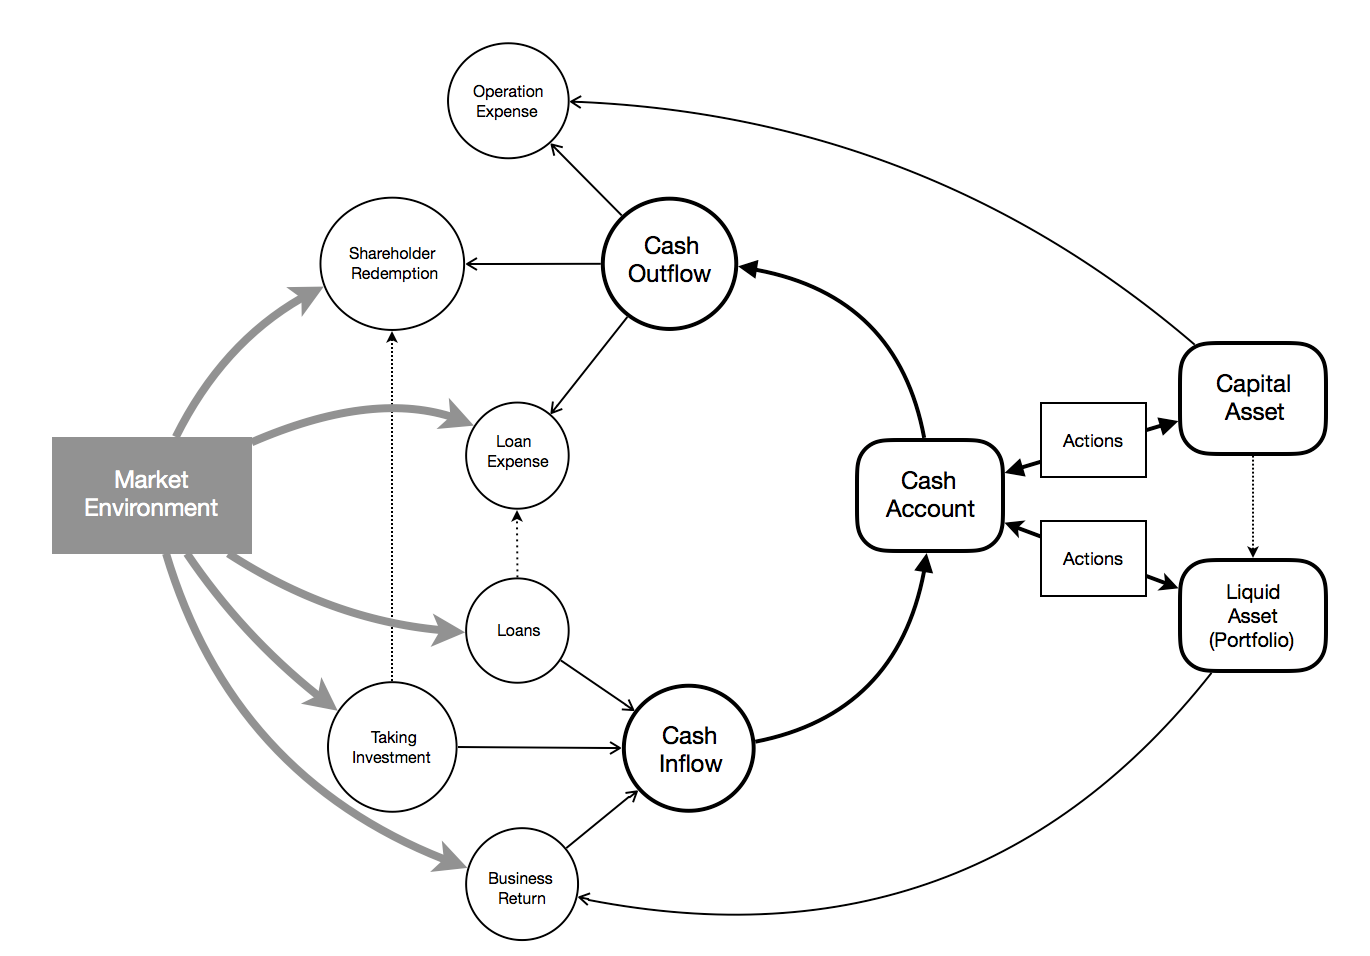
\includegraphics[scale=.2]{Holistic}
\end{center}
\caption{Cash Flows in a Holistic Model}
\label{Holistic}
\end{figure}

\subsection{A two-assets CM model}
Since the holistic model are quite complicated to solve, we start from a simple two asset model without the consideration of capital asset, loan opportunities, investment (customer deposit) opportunities or the market environment (see figure\ref{twoAsset}).

We discussed this model in our first year's research. In order to fit the real world better, we made several modifications this year. To begin with, we changed the objective function from maximising total revenue to maximising net profits: $$\max \sum^T_{t = 0}\gamma^t  \{ rr \cdot y_t - D_t - \Gamma_t - SC_t \}.$$ We made this change since net profit can describe the performance and profitability of a company better and thus maximising the net profit are normally managers' main goal. The second modification is that we adopted a transfer cost function that is partially fixed and partially proportional to the amount of transaction. This new function can be expressed by the following formula: $$\Gamma(a) =  (K_c + k_c a) \cdot 1_{\{ a < 0\}} + (K_a +k_aa)\cdot 1_{\{a>0\}}$$ where $a$ is the amount of money transferred from asset account to cash account (negative value means the other way around); $K_c$ and $K_a$ are the fixed part of the transaction cost function while $k_c$ and $k_a$ are the parameters in the proportional part. The rationale of this modification can be explained as this: In the need of cash, the manager might want to sell some illiquid asset. This action would require two different costs: a fixed cost regardless of the amount of asset he want to sell, e.g. advertising expense, salesmen's salaries etc. and a proportional cost since illiquid assets are normally sold at lower price than its true value. Similar costs apply to the disposal of cash to get profitable assets. In financial sector, brokerage commission, which is one of the main sources of transaction cost, are also normally partially fixed and partially proportional to the transaction amount.

Moreover, we added transaction cost into shortage cost. When a company faces an amount of cash demand which exceeding its current cash level, the manager has to sell enough assets to offset the cash deficit and to pay the shortage cost: $$SC = (SP + \Gamma(D-x')) \cdot 1_{\{D>x'\}}.$$ The shortage cost consists of two parts: a fixed amount of shortage penalty and the transaction cost generated by selling asset to offset cash deficit. 

At last, we allow managers to declare bankruptcy at any point of time. Once the manager declared bankruptcy, the net profit in that time period as well as the amount of both accounts will be set as zero. Figure \ref{ModifiedModel} shows one result of this model, i.e. the actions of moving money between two account. The model suggests that once the company reaches the blue area, the manager should declare bankruptcy immediately. 

\begin{figure}
\begin{center}
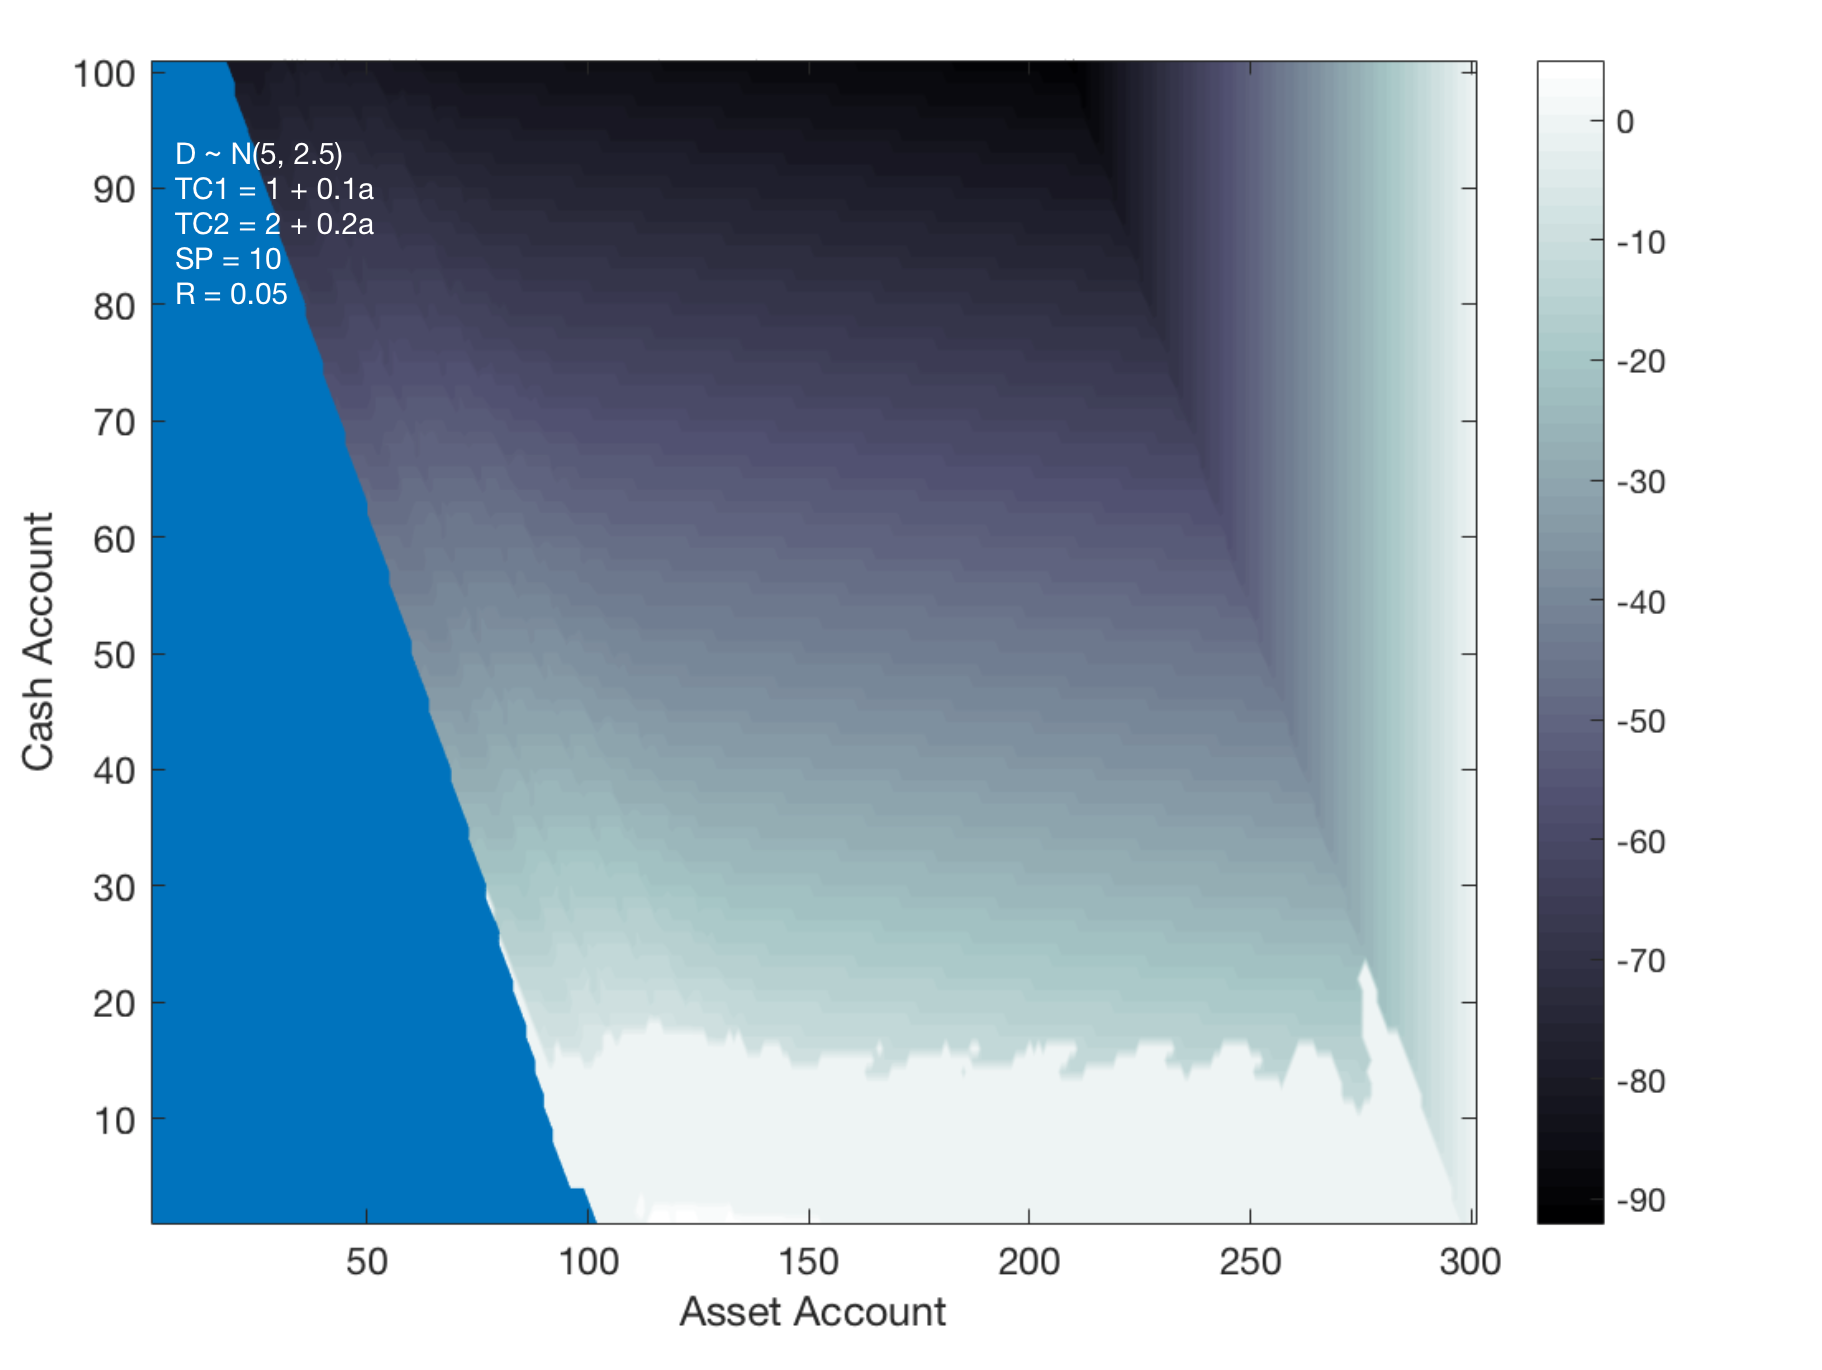
\includegraphics[scale=.3]{ModifiedModel}
\end{center}
\caption{A Optimal Solution of the Modified Model}
\label{ModifiedModel}
\end{figure}

Then we ran several simulations to evaluate the policies generated by our model. Figure \ref{simulation} shows the results of 100 simulations in four different experiments. Each experiments has the same model parameters: cash demand is normally distributed with $\mu=5.0$, $\sigma=2.5$; business return rate is $0.05$; shortage penalty is $10$ and transaction cost function has parameters $K_c = 1.0$, $k_c=0.1$,$K_a=2.0$ and $k_a=0.2$; In each simulation experiment, the manager follows the policy suggested by the dynamic programming model. The starting states for these experiments are $S = (10,90)$, $S=(10,100)$, $S=(10,110)$ and $S=(10,120)$ respectively. It can be seen that while the initial states are relatively close to each other, the results are significantly different. This suggested that in our model, given that the optimal policy is adopted, companies are highly likely to go bankrupt once they are in a `slightly bad position' (such as state 10,90) and once they are in a 'slightly good position' (such as state 10, 120) things are very unlikely to go bad.

\begin{figure}
\begin{center}
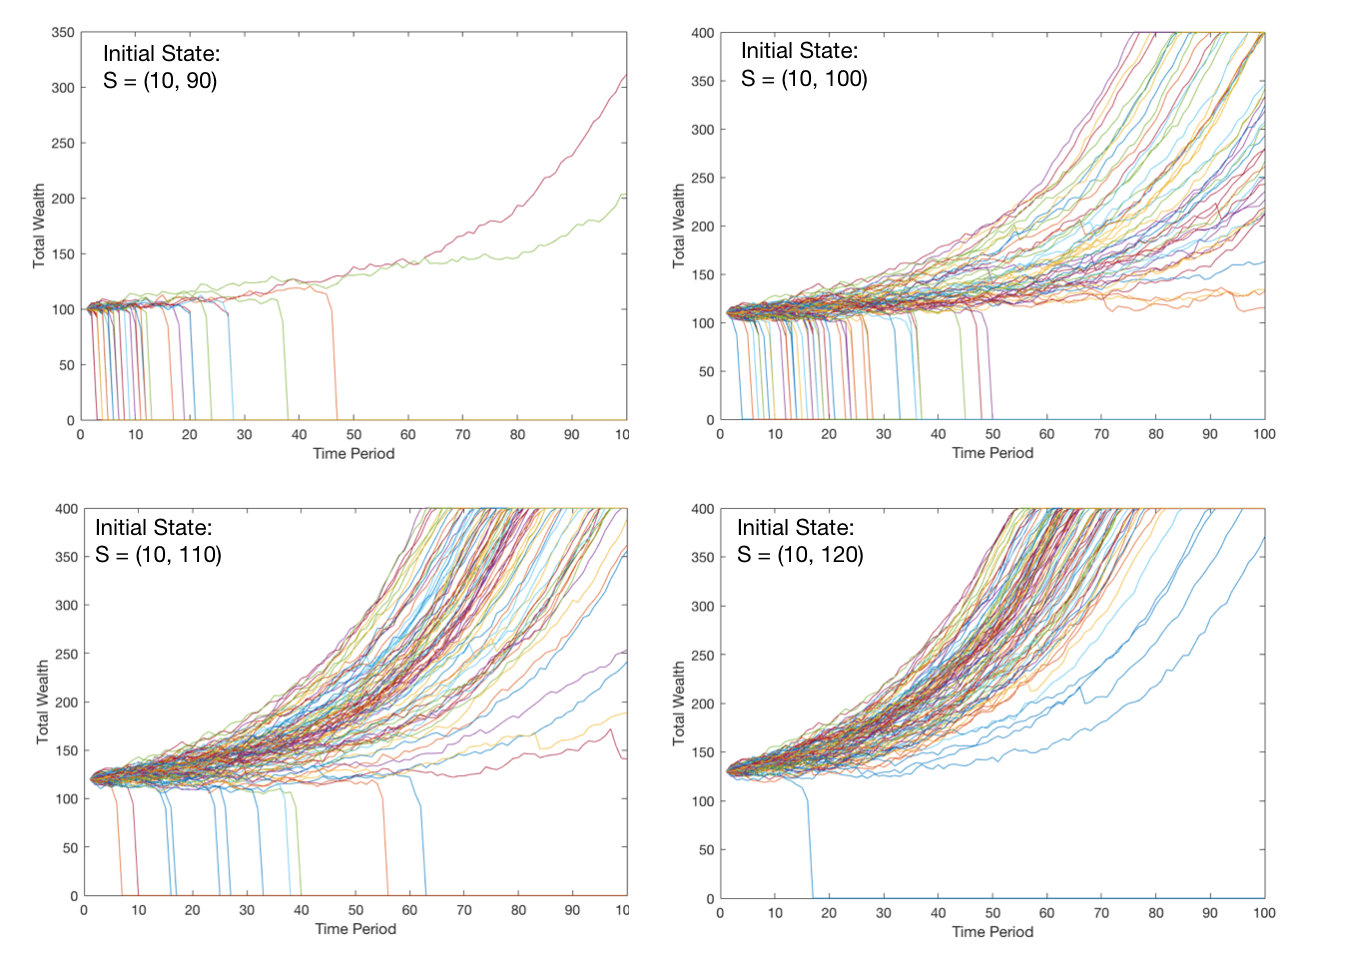
\includegraphics[scale=.56]{simu}
\end{center}
\caption{Simulation Results at Different Initial State}
\label{simulation}
\end{figure}

To examine the performance of this cash management policy more holistically, we propose a backward method to calculate the probability of going bankruptin our model. At the end the time horizon (stage 0), if the company has a non-negative cash account or has enough asset to offset its deficit, one can claim that this company does not go bankrupt (i.e. with probability 0 of going bankrupt). In other words, at stage 0, any state $S_{x, y}$ with $y \neq 0$ has value (probability of going bankrupt) equal to 0 and any state $S_{x, y}$ with $y = 0$ has value (probability of going bankrupt) equal to 1. 

At stage 1, the value of state $S_{x, y}$ equals the probability of going bankrupt in this time period plus the probability of going bankrupt in next time period (i.e. the sum of the product of the probability that the company go to stage $S_{x', y'}$ next time period (stage 0) and the value (probability of bankrupt) in that state at stage 0 for all possible $x'$ and $y'$. )

Therefore at stage 1, the probability of eventually going bankrupt for each state can be written as: 

\[
\begin{split}
V_{[x,y]}^{t=1} =& \sum P\left\{\left.S_{(0,0)}:W(S_{x,y}) = S_{(0,0)}\right|a = A^*(S_{x,y})\right\} 
\\ 
+ & \sum P\left\{ \left. S_{x',y'}:W(S_{x,y}) = S_{x',y'} \right| a = A^* (S_{x,y})\right\}  V_{[x',y']}^{t=0}
\end{split}
\]

Similarly, the value for any stage $k: k \geq 1$ can be written as

\[
\begin{split}
V_{[x,y]}^{t=k} =& \sum P\left\{\left.S_{(0,0)}:W(S_{x,y}) = S_{(0,0)}\right|a = A^*(S_{x,y})\right\} 
\\ 
+ & \sum P\left\{ \left. S_{x',y'}:W(S_{x,y}) = S_{x',y'} \right| a = A^* (S_{x,y})\right\}  V_{[x',y']}^{t=k-1}
\end{split}
\]
 
 
  Continuing this iteration until the maximum different between two successive stages' values is smaller than a small number $\epsilon =  0.0001$. In the above equations, $P\left\{ \left. S_{x',y'}:W(S_{x,y}) = S_{x',y'} \right| a = A^* (S_{x,y})\right\}$ is the probability that the company goes from state  $S_{x,y}$ to $S_{x',y'}$ when the manager follows the optimal policy $A^*$.
  
Figure \ref{prob} shows the probability of going bankrupt when a company follows the optimal cash management policy. The right graph is the result calculated by the recursive method proposed above. The left graph is the probability of going bankrupt generated by 10,000 simulations. It can be seen that the two results are quite similar: both probabilities jump from $1.0$ to $0.0$ very quick. This result suggest that once the optimal cash policy is adopted, most companies will either go to bankrupt or go to a `safe position' where it is almost impossible for the companies to get worse, depending on which states are they currently in.



\begin{figure}
\begin{center}
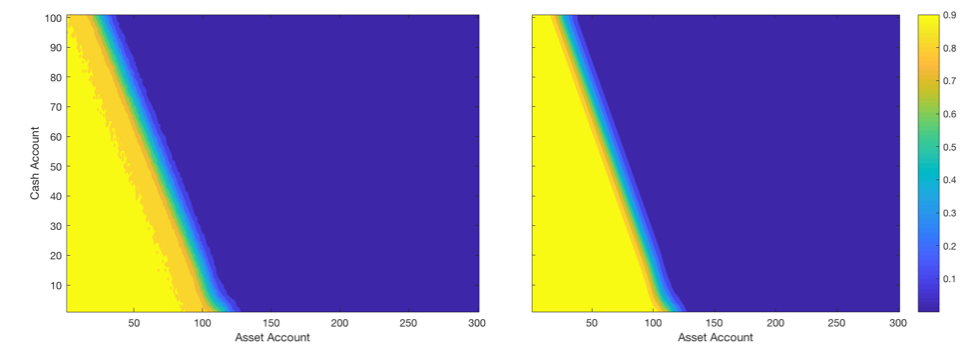
\includegraphics[scale=.40]{prob}
\end{center}
\caption{Probabilities of Going Bankrupt in Each State}
\label{prob}
\end{figure}






\subsection{Cash management with loans/investment}
As we discussed in the former section, the optimal cash management policy could help those companies currently in `good position' get to a safe status where it is almost impossible for companies to go bankrupt. However, once companies get into a `bad position' where their business revenue cannot cover the cash demand, managers has to sell his asset to meet the current demand, which would deteriorate the companies' profitability further. 

In reality, however, once companies' income could not cover its cash demand, instead of selling asset and jeopardising future profitabilities, managers tend to take loans from other companies or financial intermediaries. In light of this, we propose a two-asset accounts model with loan options. Figure \ref{loan} shows the basic idea of this model. 

\begin{figure}
\begin{center}
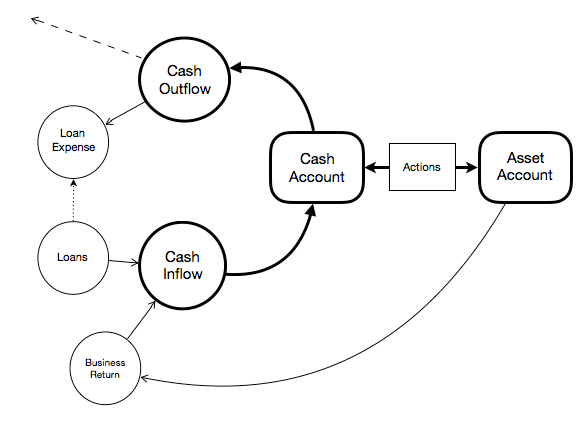
\includegraphics[scale=.43]{loan}
\end{center}
\caption{Two Asset Accounts Model with Loan Options}
\label{loan}
\end{figure}

In addition to the normal two asset accounts model, we add a `taking loan' option in the model i.e. at any point of time, the manager could take a loan from financial companies. Once a loan was taken, a certain amount of loan repayment must be paid in every following time period until the debt (loan and interest) is offset.   

For simplicity's sake, we assume that there is only one type of loans available in the market and a company is not allowed to take another loan while its debt has not been offset. Let the loan size be $L$ and the interest rate be $lr$. We also assume that once the loan is taken, one must pay a fixed amount $LP$ in each one of the following $N$ time periods. So in each time period, the loan expense can be written as: $$LP = L \cdot \frac{lr \cdot (1+lr)^N}{(1+lr)^N-1}$$
 
 We also formulated this model as a Markov Decision Process where each state consists of three parameters: $S_{x,y,z}$ where $x$ and $y$ represent the current cash and asset level and $z$ represent the remaining times of loan repayment. For example, at time period $t$, a manager takes the loan. Then at time $t+1$ the $z$ value of the company's state changes from $0$ to $N$. In the following periods, the company's cash demand will increase by $LP$ amount and after each period, $z$ value will decrease by $1$ until it gets to $0$. Moreover, the action space also need some modification. Now the action space consists of two parameters: $a_c$ (the amount of money transfer between cash and asset) and $a_l$ (can only take values 0 or 1, indicating whether take the loan or not). Since we assumed that one cannot take loans had his debt not been fully paid, $a_l$ cannot take the value of 1 when $z \neq 0$.
 




One limitation of using Markov Decision Process to solve the cash management model with loan options is the high calculation cost. It took more than 10 hours to get the optimal solution with the assumption of one loan available. To expand the model to a model with multiple loan options, the calculation time will growth exponentially. Thus we propose a heuristic method called one-step policy improvement to get an approximate solution.
\begin{figure}
\begin{center}
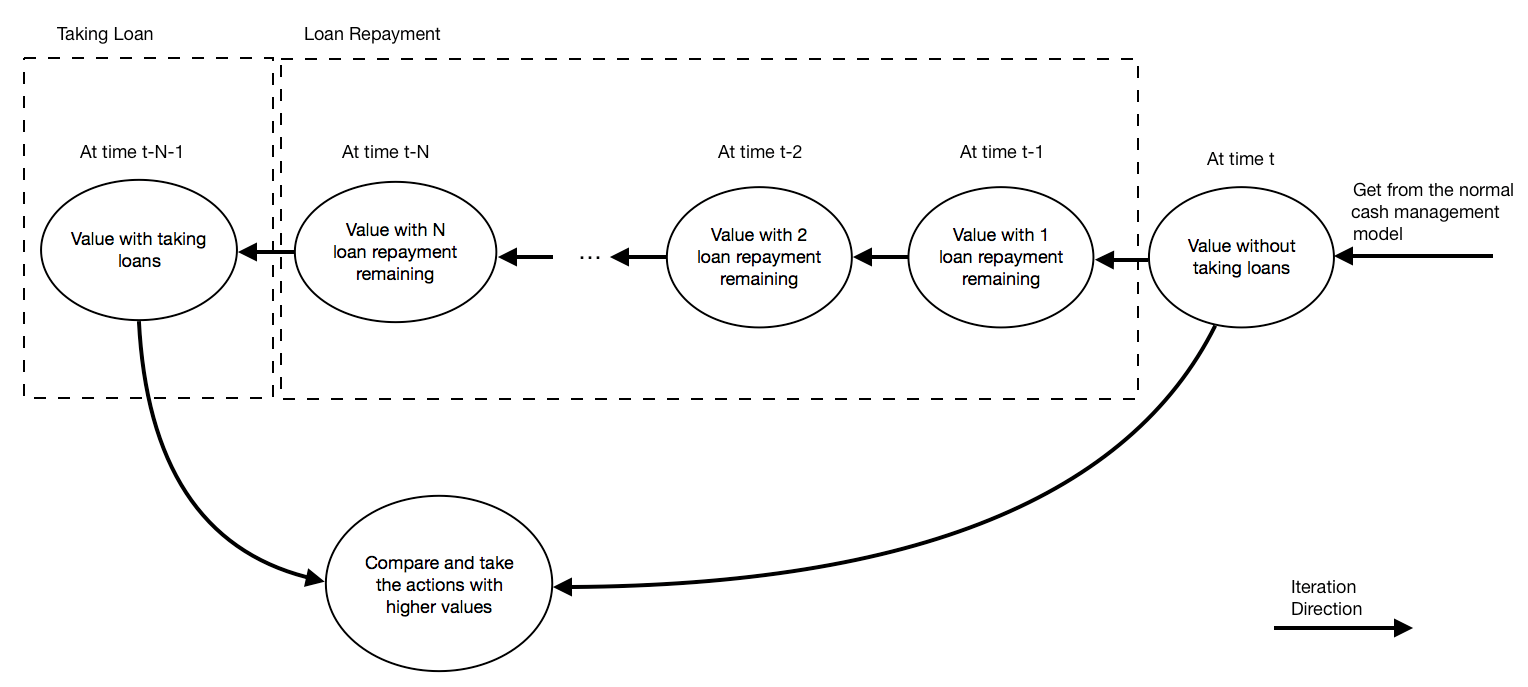
\includegraphics[scale=.28]{oneImprov}
\end{center}
\caption{One Improvement Policy}
\label{oneImprov}
\end{figure}

The basic idea of one-step policy improvement is shown in figure \ref{oneImprov}. The main task is to calculate the value of each cash-asset state conditioning on that the manager has decided to takes loans in the current time period and will never takes loan again. The value of state $S_{x,y}$ given the fact that the manager has decided to take the loan at the current time period and will follow the optimal cash management action $a'_c$ can be denoted by the notation: $$V^{{a_c}', a_l = 1}(S_{x,y}).$$
Then compare this value with the value in the same state but without taking loans in the whole time planning horizon, denoted by the notation: $$V^{{a_c}, a_l = 0}(S_{x,y}).$$ where $a_c$ is the optimal cash management policy without any loan opportunity. So this strategy is the same with the cash strategy from the normal Cash DP model ($a$). Correspondingly, the value $V^{{a_c}, a_l = 0}(S_{x,y})$ is the same with the value from the normal Cash DP model $V^a(S_{x,y}).$


In the normal Cash DP model, we have that $$V^{a_c, a_l =0}(S_{x,y})= V^a(S_{x,y}) =    \gamma R_t^{a}(S_{x,y}) + \gamma \sum_{S_{x',y'}\in S} V^{a}_{t-1}(S_{x',y'})
\mathbb{P}\left\{S_{x',y'}:W(S_{x, y}) = S_{x', y'} \right\}$$

In the above equation, $R^{a}_t(S_{x,y})$ is the return function and can be represent as:$$ R^{a}_t(S_{x,y}) = rr*y - \Gamma(a) - \mathbb{E}[D+SP(S_{x,y},a)]$$


We define $N$ as the total number of times of loan repayment one has to make. $a_{c, z}$ is the optimal cash management action when there is $z$ loan repayments left,  $L$ is the size of the loan and $lr$ is the corresponding loan interest rate. So we have 

$$V^{a_c', a_l = 1}(S_{x,y}) = L+R^{a}(S_{x+L,y}) + \gamma \sum_{S_{x',y'}\in S }V^{a_{c,z=N}}(S_{x',y'}) \mathbb{P}\left\{ S_{x',y'} : W(S_{x+L,y}=S(x',y')\right\}$$



Let $LP$ be the loan payment in each time period. Now the value of  $V^{a_{c,z=N}}(S_{x+ls, y})$ could be calculated recursively: 
$$a_{c,1} = \arg \max_{a_{c,1} \in \Pi} \gamma [R^{a_{c,1}} (S_{x,y}) - LP] + \gamma  \sum_{S_{x',y'}\in S} V^a(S_{x',y'})\mathbb{P}\left\{S_{x',y'}\widehat{W}(S_{x-LP, y}) = S_{x', y'} \right\}$$
$$ V^{a_{c,1}}(S_{x,y}) = \gamma [R^{a_{c,1}} (S_{x,y}) - LP] + \gamma  \sum_{S_{x',y'}\in S} V^a(S_{x',y'})\mathbb{P}\left\{S_{x',y'}:\widehat{W}(S_{x-LP, y}) = S_{x', y'} \right\}$$

$$a_{c,2} = \arg \max_{a_{c,2} \in \Pi} \gamma  [R^{a_{c,2}} (S_{x,y}) - LP]  + \gamma  \sum_{S_{x',y'}\in S} V^{a_{c,1}}(S_{x',y'}) \mathbb{P}\left\{S_{x',y'}:\widehat{W}(S_{x-LP, y}) = S_{x', y'} \right\}$$
$$ V^{a_{c,2}}(S_{x,y}) = \gamma  [R^{a_{c,2}} (S_{x,y}) - LP]   + \gamma  \sum_{S_{x',y'}\in S} V^{a_{c,1}}(S_{x',y'}) \mathbb{P}\left\{S_{x',y'}:\widehat{W}(S_{x-LP, y}) = S_{x', y'} \right\}$$

$$...$$

$$a_{c,N-1} = \arg \max_{a_{c,N} \in \Pi} \gamma [R^{a_{c,N-1}} (S_{x,y}) - LP] + \gamma  \sum_{S_{x',y'}\in S} V^{a_{c,N-2}}(S_{x',y'}) \mathbb{P}\left\{S_{x',y'}:\widehat{W}(S_{x-LP, y}) = S_{x', y'} \right\}$$
$$ V^{a_{c,N-1}}(S_{x,y}) = \gamma [R^{a_{c,N-1}} (S_{x,y}) - LP] + \gamma  \sum_{S_{x',y'}\in S} V^{a_{c,N-2}}(S_{x',y'}) \mathbb{P}\left\{S_{x',y'}:\widehat{W}(S_{x-LP, y}) = S_{x', y'} \right\}$$

$$a_{c,N} = \arg \max_{a_{c,N} \in \Pi} \gamma [R^{a_{c,N}} (S_{x,y}) - LP] + \gamma  \sum_{S_{x',y'}\in S} V^{a_{c,N-1}}(S_{x',y'}) \mathbb{P}\left\{S_{x',y'}:\widehat{W}(S_{x-LP, y}) = S_{x', y'} \right\}$$
$$ V^{a_{c,N}}(S_{x,y}) = \gamma [R^{a_{c,N}} (S_{x,y}) - LP] + \gamma  \sum_{S_{x',y'}\in S} V^{a_{c,N-1}}(S_{x',y'}) \mathbb{P}\left\{S_{x',y'}:\widehat{W}(S_{x-LP, y}) = S_{x', y'} \right\}.$$

Then for each state, we compare the value of `taking loan once and never take it again' i.e. $V^{a'_c,a_l = 1}(S_{x,y})$ with the value of `not taking loan in the entire planning time horizon' i.e. $V^a(S_{x,y})$. For any state $S_{x,y,z=0}$, if the policy `taking loan once and never take it again' is better than `not taking loan at all', then whenever the system comes to the state $S_{x,y,z=0}$, the loan should be taken.

Then we examine the performance of the one step improvement algorithm using simulation method. Based on the old model settings, we assume that the manager could take a loan with size 40, loan interest rate 0.03. Once the loan is taken, it should be paid within 40 time periods with equal amount of repayment in each time. Figure \ref{OSI} shows the total number of identical companies that did not declare bankrupt in each time period during total 10,000 simulations. It can be seen that the probabilities for a company not going bankrupt can be increased when the loan is available on the financial market. Moreover, the performance of the policy suggested by the one-step policy improvement algorithm is quite close to the policy suggested by the dynamic programming method. With respect to calculation time, dynamic programming would take more than 10 hours while the one-step improvement algorithm only take 8 minutes on the same PC. 

Furthermore, with one-step improvement algorithm, one could easily expand the cash management model with single loan option to a model with multiple loan options. Assume there are two possible loan options, i.e. $a_l$ could take value of $0$, $1$ and $2$. Let $a_l = 0$ represent that the manager does not take any loans, $a_l=1$ represent that he takes the first loan and do not take any loan thereafter and $a_l=2$ represent that he takes the second loan and do not take any loan thereafter. By using one-step policy improvement, one need to calculate $V^{a'_c, a_l=1}(S_{x,y})$ and $V^{a'_c, a_l=2}(S_{x,y})$ separately for each state $S_{x,y}$. Then for each state, the highest value among $V^a(S_{x,y})$, $V^{a'_c, a_l=1}(S_{x,y})$ and $V^{a'_c, a_l=2}(S_{x,y})$ should be recorded along with its corresponding actions. The recorded policy is the policy suggested by one-step policy improvement algorithm. 


\begin{figure}
\begin{center}
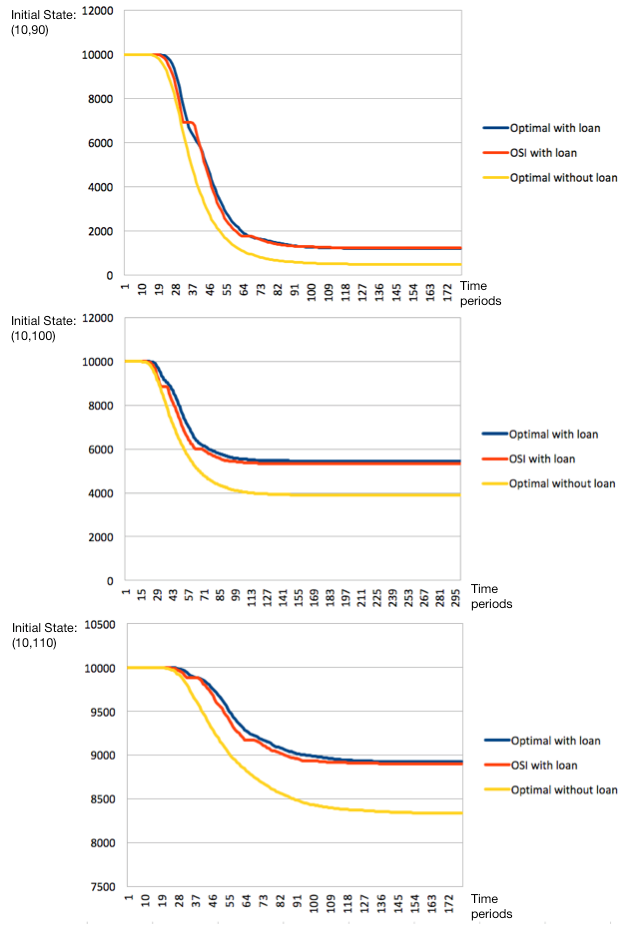
\includegraphics[scale=.6]{OSI}
\end{center}
\caption{Survival Companies with Different Policies}
\label{OSI}
\end{figure}

\subsection{Approximate dynamic programming}
In DP, we initialise the values of each state at stage 0 (i.e. at the end of the planning time horizon) as zero. Then recursively we update the optimal action set and the optimal value set using the update rule:
$$a(S_{x,y}) = \arg\max \left\{   
R_t^{a}(S_{x,y}) + \gamma \sum_{S_{x',y'}\in S} V^{a}_{t-1}(S_{x',y'})
\mathbb{P}\left\{S_{x',y'}:W(S_{x, y}) = S_{x', y'} \right\}
 \right\} $$
$$V^a(S_{x,y}) =  R_t^{a}(S_{x,y}) + \gamma \sum_{S_{x',y'}\in S} V^{a}_{t+1}(S_{x',y'})
\mathbb{P}\left\{S_{x',y'}:W(S_{x, y}) = S_{x', y'} \right\}.$$
One limitation of applying dynamic programming is its complexity of the algorithm. The CM model with loan options or the holistic model are too complicated to apply dynamic programming method. One possible way to solve these models is to use approximate dynamic programming instead. To get a better understanding of ADP and also to examine how ADP performs in cash management models, we first applied one of the ADP methods named temporal-difference learning (TD) in the simple two assets model. In this method, we simulate the situation for one time period and record its immediate reward. Then we update the value for the state based on the immediate reward and the value for the state we recorded before the simulation. For example, if currently the company is in the state $S_{x,y}$ and following a specific policy $\pi$ (say the $\epsilon$-greedy policy i.e. the policy will suggest the action which gives the highest state value with probability $1-\epsilon$ and will suggest a random action with probabiliy $\epsilon$) which suggesting action $a^{\pi}(S_{x,y})$. We simulate the situation and get the current net profit $R$ and the state where the company will be in next time period $S_{x',y'}$. Then we can update the value of state $V(S_{x,y}|A=a^\pi(S_{x,y}))$ as: 
 $$V(S_{x,y}|A=a^\pi(S_{x,y})) + \alpha \left[ R + \gamma V(S_{x',y'}|A=a^\pi (S_{x',y'}))\right] - V(S_{x,y}|A=a^\pi(S_{x,y}))$$ where $\alpha$ is the update step size parameter. Then we repeat this step until the value converges. In this method we only simulate for one time period (1-step $TD$, see figure \ref{oneStep}). To improve the performance of this algorithm (i.e. the rate of convergence), we could also simulate it for more than one time period (n-step $TD$, see figure \ref{nStep}). Assume that the company reaches a terminal state (a state indicating bankruptcy or a state with maximum cash and asset) in T time periods, then a T-step $TD$ method is equivalent to Monte Carlo simulation. 
 \begin{figure}
\begin{center}
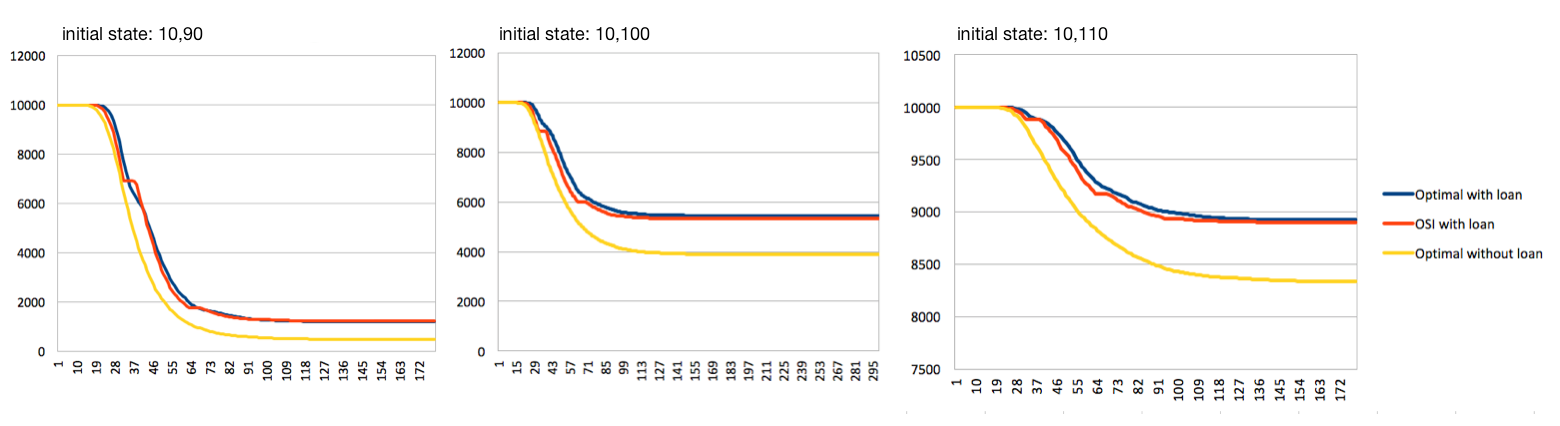
\includegraphics[scale=.4]{oneStep}
\end{center}
\caption{1-step $TD$ Method}
\label{oneStep}
\end{figure}


\begin{figure}
\begin{center}
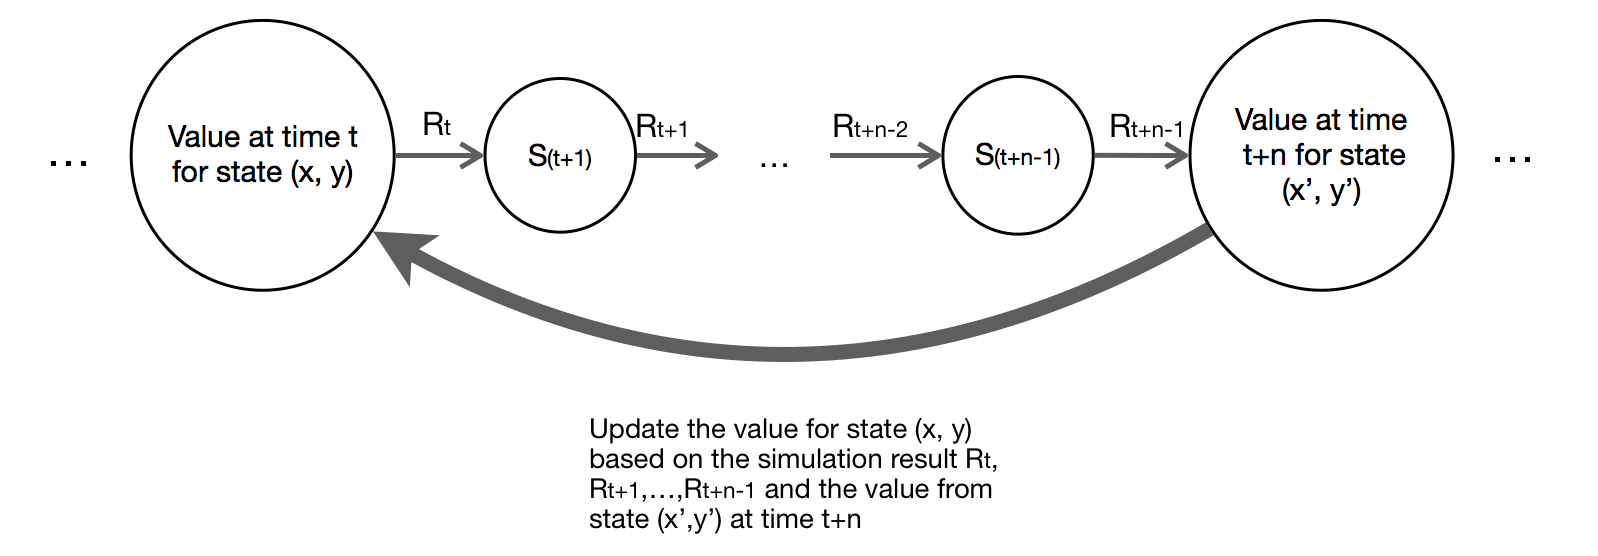
\includegraphics[scale=.4]{nStep}
\end{center}
\caption{n-step $TD$ Method}
\label{nStep}
\end{figure}

Moreover, we also intend to use Eligibility Trace method which provide a way of shifting and choosing between Monte Carlo and each step $TD$ methods. The ET method could be viewed as a weighted average of $1$-step $TD$, $2$-step $TD$, ... , $T$-step $TD$. The weight for $i$-step $TD$ is $(1-\lambda) \lambda ^ {i-1}$. The coding and the numeric experiments for applying eligibility trace into the cash management model is still ongoing.

We also intend to use function approximation to solve these CM models, i.e looking for a function to approximate the value for each state. This would help us convert the discrete states model into a continuous states model which fits better in cash management problem.



\section{Research plan for next year}

The research for next year mainly consists of four parts: 
\begin{itemize}
\item Study temporal difference and eligibility trace method and apply it into cash management models
\item Study approximate functions in ADP; Find a function that can approximate values in DP model.
\item Read more literature about cash flows in financial companies and modify the holistic model.
\item Do numeric experiments for each cash management model and finish the thesis.
\end{itemize}
The specific study plan can be seen in the table \ref{Plan}



\begin{table}

\centering
\begin{tabular}{| l | l |}
\hline
\hline
September & Use ET in two assets model;\\
\hline
October & Numeric experiment of two assets model;\\
& Study the function approximate in ADP;\\
\hline
November & Continue in the study of the function approximate in ADP;\\

& Write the fourth chapter of the thesis;\\
\hline
December & Finish the fourth chapter of the thesis;\\
& Continue in the study of the function approximate in ADP;\\
\hline
January & Use TD and ET in the CM model with loans;\\
& Write the fifth chapter of the thesis;\\
\hline
Feburary & Use Approximate Functions in the CM model with loans;\\
& Write the fifth chapter of the thesis;\\
\hline
March & Numeric experiment of the CM model with loans\\
& Finish the fifth chapter of the thesis;\\
\hline
April & Read more literature about cash flows in financial sector\\
& Modify the holistic model\\
\hline
May & Read more literature about cash flows in financial sector;\\
& Use TD and ET in the holistic model\\
\hline
June & Write up the sixth chapter of the thesis\\
& Use approximate functions in the holistic model\\
\hline
July & Write up the sixth chapter of the thesis\\
& Numeric experiment in the holistic model\\
\hline
August & Finish the sixth chapter of the thesis;\\
& Write the literature review of the thesis;\\
\hline
September & Write the methodology of the thesis;\\
& Finish the first draft of the thesis;\\

\hline
\hline
\end{tabular}
\caption{Next Year Research Schedule}
\label{Plan}
\end{table}


\section{Courses and activities}
In last year, I took one NATCOR course, Simulation in Loughborough University and passed with $86\%$. I also took one APTS course, Applied Stochastic Process and Statistical Modelling in Oxford University (no assessment). I also learned how to use HEC in the university which helps me a lot in the model computation. Moreover, I helped in teaching MNGT 130: Introduction to Business Analytics, MSCI 212: Statistical Methods for Business and MSCI 224: Techniques for Management Decision Making. I benefit a lot from the above study activities and the teaching experience is invaluable.

Next year I am going to take another NATCOR course, Combinatorial Optimisation (in September 2017). Moreover I will give a presentation about my research to MSCI stuff and PhD students in Lancaster University. I will also participate two conferences, presumably one of them is the StochMod 2018 at Lancaster University.



\newpage
\bibliographystyle{plain}
\bibliography{BibliographyinCashProblem}
%\end{spacing}
\end{document}